\chapter{Estado de la Cuestión}
\label{cap:estadoDeLaCuestion}


Los humanos siempre  han tenido la necesidad inherente de comunicarse y quien no es capaz de hacerlo, generalmente acaba excluido. A día de hoy este problema sigue afectando a parte de la población como es el caso de las personas con Trastorno del Espectro Autista (\textit{TEA}).
\\

Sin entrar en gran detalle, podemos encontrar que la gente con \textit{TEA} tienen dificultades en la comunicación verbal, pues a menudo ésta no es recíproca o no se realiza en el contexto social adecuado. Respecto a la comunicación no verbal, también sufren dificultades al entender el significado de gestos faciales o expresión corporal de otras personas. Todo esto causa a menudo malentendidos, pues generalmente no se comprende el contexto y dificulta la comunicación. 


\section{Sistemas Aumentativos y Alternativos de Comunicación}
Los Sistemas Aumentativos y Alternativos de Comunicación (\textit{SAAC}) son las distintas formas de expresión sin tener en cuenta el lenguaje hablado que tiene como finalidad aumentar y/o compensar los problemas de comunicación de personas con discapacidad como por ejemplo trastornos del espectro autista, discapacidad intelectual, deficiencia auditiva, parálisis cerebral entre otros.

En ocasiones puede hacer falta el uso de recursos para poder comunicarse, es por ello que podemos distinguir dos tipos de \textit{SAAC}, los sistemas sin ayuda y los sistemas con ayuda.
\newpage
\begin{itemize}
	\item \textbf{Sistemas sin ayuda}: no utilizan ningún recurso externo para establecer una comunicación, únicamente usan su propio cuerpo. En los sistemas sin ayuda podemos observar dos tipos de grupos, los métodos gestuales (lengua de signos) y los métodos oralistas (lectura labiofacial). 
	\item \textbf{Sistemas con ayuda}: utilizan recursos externos para establecer una comunicación. Los más utilizados suelen ser pictogramas, imágenes o símbolos.
\end{itemize}

Las \textit{SAAC} utilizan múltiples recursos para poder comunicarse con personas con discapacidades cognitivas y entre todos ellos destacan los sistemas pictográficos. Se trata de uno de los sistemas más utilizados y esto es debido a su fácil comprensión ya que representan gráficamente lo que se desea transmitir como palabras o conceptos. 

\section{Pictogramas}
Los pictogramas son imágenes o símbolos de rápida comprensión que expresan acciones, objetos, emociones etc. Un conjunto de pictogramas en orden, puede generar una oración. Todos ellos deben cumplir las siguientes características:
\begin{enumerate}
	\item \textbf{Referencialidad}: Busca la relación del pictograma con el referente.
	\item \textbf{Ítems gráficos}: imágenes que representen de manera sencilla aquello que se toma como modelo.
	\item \textbf{Comprensión}: debe ser fácilmente entendible independientemente de la formación, idioma o discapacidad.
	\item \textbf{Legibilidad}: Mantiene una coherencia visual entre pictogramas.
	\item \textbf{Sencillez}: Muestra únicamente los elementos relevantes sin elementos distractores o adornos insignificantes.
\end{enumerate}

\subsection*{Sistemas pictográficos}
Los sistemas pictográficos 
Existen numerosos sistemas pictográficos a continuación hablaremos de los más importante:

\subsection{Sistema pictográfico de comunicación - SPC}

Creado en 1981 por Roxana Mayer Johnson con la intención de facilitar la comunicación a quienes tienen un nivel de lenguaje expresivo simple o vocabulario limitado. Gracias a la diferenciación por colores, facilita la comprensión de la estructura sintáctica. Está organizado por seis colores según su función gramatical. Actualmente cuenta con más de 3000 iconos.

\begin{itemize}
	\item \textbf{Personas} (Amarillo): Representa a familiares y pronombres. Ejemplo: Mamá, familia,  yo, ellos.
	\item \textbf{Verbos} (Verde): Representan acciones. Ejemplo: Abrir, agarrar, comer, ir.
	\item \textbf{Descriptivos} (Azul): Descriptivos o adjetivos o adverbios
	\item \textbf{Nombre} (Naranja): Representan objetos u otros elementos que no aparecen en otra categoría. Ejemplo: Gato, Almohada o Casa.
	\item \textbf{Miscelánea} (Blanco): Representa números, letras y colores
	\item \textbf{Social} (Rosa): Vocabulario relacionado con relaciones sociales. Ejemplo: Buenos días, si, gracias, no lo sé.
	
\end{itemize}

\footnote{\url{https://www.uv.es/bellochc/logopedia/NRTLogo8.wiki?8}}

% TODO: \usepackage{graphicx} required
\begin{figure}[h!]
	\centering
	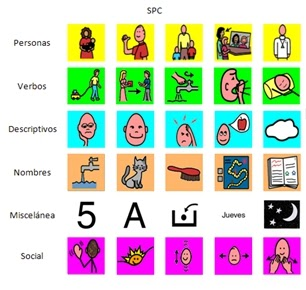
\includegraphics[width=0.7\linewidth]{Imagenes/Bitmap/SPCcolores}
	\caption{Ejemplo de categorías en Sistema Pictográfico de Comunicación.}
	\label{fig:spccolores}
\end{figure}

\subsection{Blissymbolics}
Está compuesto por más de 5.000 símbolos (\textit{Bliss-word}) los cuales a su vez están formados por uno o más caracteres Bliss (\textit{Bliss-Character}). Para poder comprender los símbolos es necesario conocer el significado de los \textit{Bliss-Character} que rondan los 150, siendo de fácil comprensión.

 Destacar que el orden, el tamaño o la posición de los símbolos puede alterar el significado del símbolo. Adicionalmente pueden estar agrupados por colores descritos en SPC.
\footnote{\url{https://www.blissymbolics.org/index.php/about-blissymbolics}}

% TODO: \usepackage{graphicx} required
\begin{figure}[h!]
	\centering
	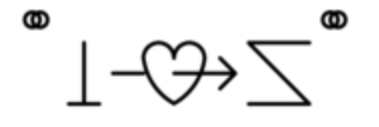
\includegraphics[width=0.3\linewidth]{Imagenes/Bitmap/Blissymbolics}
	\caption[Ejemplo Blissymbolics]{En la imágen podemos ver “Amante de bliss” como la combinación de persona (T invertida), amar y bliss (Z invertida).}
	\label{fig:blissymbolics}
\end{figure}


\subsection{Sclera}
La principal característica de Sclera frente a otros sistemas pictográficos es que sus pictogramas son menos coloridos pero cuentan con pictogramas más avanzados en cuanto a acciones que representan. Cuenta con un total de 11497 pictogramas en español.

En la actualidad el funcionamiento de Sclera está paralizado desde 2015.
\footnote{\url{https://www.sclera.be/en/picto/cat/12}}
\footnote{\url{http://aulaabierta.arasaac.org/pictograma-de-sclera}}

% TODO: \usepackage{graphicx} required
\begin{figure}[h!]
	\centering
	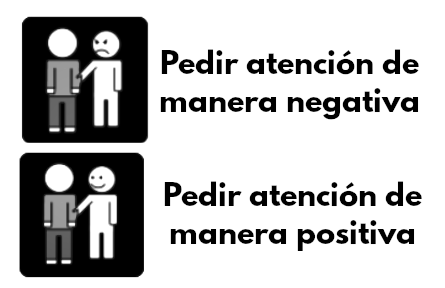
\includegraphics[scale=0.34]{Imagenes/Bitmap/Sclera}
	\caption{Ejemplo de acciones en Sclera.}
	\label{fig:sclera}
\end{figure}

\newpage
\subsection{Mulberry}
Mulbery se creó con el propósito de ser un sistema pictográfico orientado a adultos ya que un gran porcentaje de dichos sistemas estaban pensados principalmente para niños y dificultaban la comunicación por falta de pictogramas.

Los pictogramas de Mulbery cuentan con 118 categorías incluyendo sustantivos, pronombres, verbos y con un total de 3436 pictogramas.
\footnote{\url{https://mulberrysymbols.org/}}


% TODO: \usepackage{graphicx} required
\begin{figure}[h!]
	\centering
	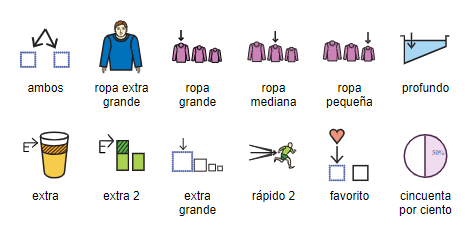
\includegraphics[scale=0.7]{Imagenes/Bitmap/Mulberry}
	\caption{Ejemplo de pictogramas de Mulberry.}
	\label{fig:mulberry}
\end{figure}

\newpage
\subsection{Minspeak}
Es un sistema de comunicación alternativo creado por Bruce Baker en 1982. Difiere con los vistos anteriormente en que el significado de los iconos no viene preestablecido sino que es acordado entre usuario y logopeda. Es por ello que cada icono acordado tenga un significado distinto según la secuenciación de iconos.

Para generar la relación entre icono se hacía uso de Programas de Aplicación Minspeak (\textit{PAM}) que es un tablero en el cual están todos los iconos y según el presionado, se iluminarán los otros iconos que permitan formar una secuencia por estar vinculados.

\footnote{\url{http://ares.cnice.mec.es/informes/18/contenidos/94.htm}}
% TODO: \usepackage{graphicx} required
\begin{figure}[h!]
	\centering
	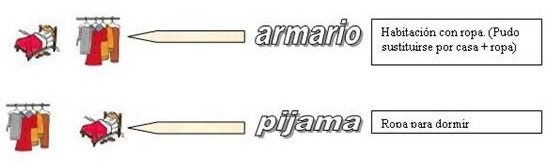
\includegraphics[width=0.7\linewidth]{Imagenes/Bitmap/Minspeak}
	\caption{Ejemplo de Minspeak.}
	\label{fig:minspeak}
\end{figure}


\subsection{ARASAAC}

El portal Aragonés de Comunicación Aumentativa y Alternativa (ARASAAC) surge en 2007 gracias a la colaboración entre el personal del CATEDU, el colegio público de educación Especial Alborada y del Centro Politécnico Superior. Su objetivo era la creación de un sistema pictográfico de libre distribución que ayudaran en el ámbito de la comunicación a todas aquellas personas que lo necesitasen.
Actualmente el portal de ARASAAC incluye fotografias, videos y cuenta con más de 39000 pictogramas tanto a color como en blanco y negro y con traducciones a 20 idiomas. También ofrece herramientas online con las que poder generar materiales como por ejemplo generador de calendarios, generador de tableros, creador de símbolos, etc.

A diferencia de otros sistemas pictográficos ARASAAC permite una gran cantidad de opciones configurables como el color de fondo, marco o tiempo verbal.

\footnote{\url{http://www.arasaac.org/}}
\footnote{\url{http://carei.es/descipcion-arasaac/}}

\begin{figure}[h!]
	\centering
	\includegraphics[width=0.7\linewidth]{Imagenes/Bitmap/Configuarción ARASAAC}
	\caption{Opciones de configuración de un pictograma.}
	\label{fig:configuarcion-arasaac}
\end{figure}



También cabe destacar que ARASAAC ha recibido varios premios por su labor y que es una herramienta utilizada en varios países por lo que la cantidad de usuarios que colaboran es muy alta, esto queda reflejado en la cantidad de pictogramas que se publican a la plataforma por parte de colaboradores sin ningún ánimo de lucro, dichos pictogramas están constantemente actualizándose. Un ejemplo de ellos son los pictogramas que se han publicado debido a la pandemia.

\newpage
% TODO: \usepackage{graphicx} required
\begin{figure}[h!]
	\centering
	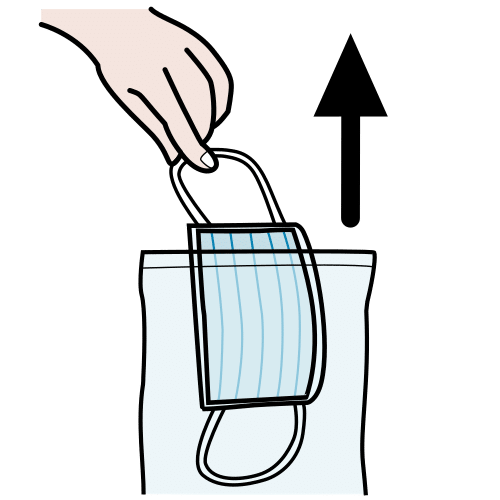
\includegraphics[width=0.2\linewidth]{Imagenes/Bitmap/Picto Mascarilla}
	\caption{Acción de sacar la mascarilla.}
	\label{fig:picto-mascarilla}
\end{figure}

\begin{figure}[h!]
	\centering
	
\includegraphics[width=0.2\linewidth]{Imagenes/Bitmap/Mascarilla mal colocada}
	\caption{Pictograma que representa mascarilla mal colocada.}
	\label{fig:picto-mascarilla-mal-colocada}
\end{figure}

\section{Editores de Tableros basados en Pictogramas}

A menudo estos tableros se realizan mediante piezas de papel recortadas y trabajar con ellas puede resultar engorroso, poco eficiente y apenas permiten modificaciones. Es por ello que la evolución lógica de los tableros pictográficos ha sido la digitalización. Para crear y editar tableros se han creado multitud de aplicaciones, a continuación estudiaremos sus características.

\subsection{Pictoselector}
Es una herramienta gratuita para crear agendas visuales. Recopila más de 28.000 provenientes de \textbf{Sclera}, \textbf{Mulberry}, \textbf{ARASAAC}, etc. Al crear un proyecto, permite cargar una plantilla o crear una desde cero. Se puede modificar el número de filas y columnas, la posición del texto y el tamaño del borde de los pictogramas.
\footnote{\url{ https://www.pictoselector.eu/es/ }}

% TODO: \usepackage{graphicx} required
\begin{figure}[h!]
	\centering
	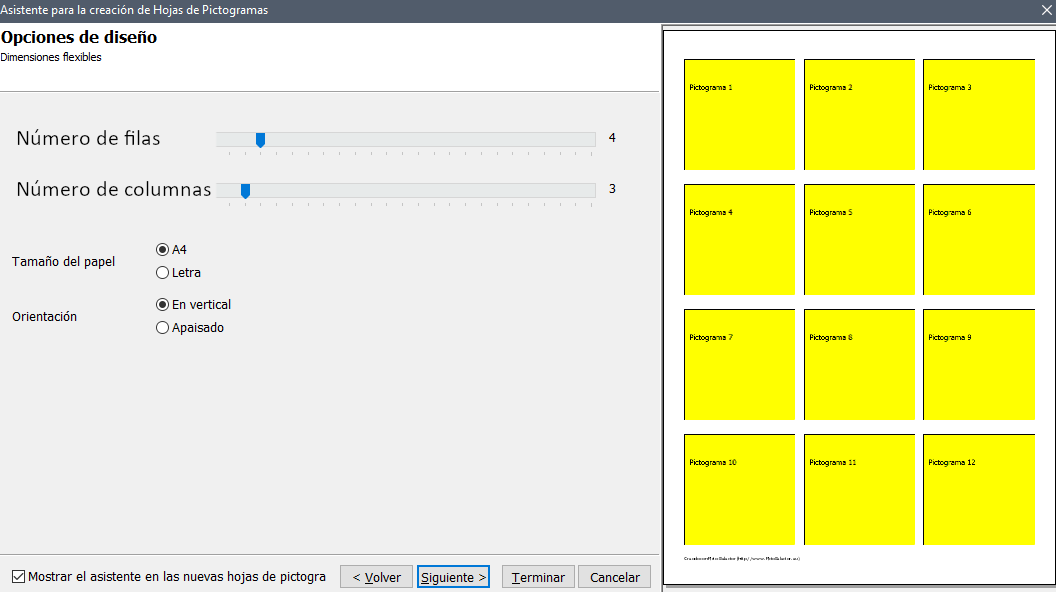
\includegraphics[width=0.7\linewidth]{Imagenes/Bitmap/Pictoselector Tablero}
	\caption{Ventana donde se edita el tamaño de la cuadrícula.}
	\label{fig:pictoselector-tablero}
\end{figure}


Una vez creado el tablero, podemos insertar en su cuadrícula distintos elementos, muchos de ellos en forma de pictograma. Para facilitar esta tarea, la cabecera de la aplicación contiene acceso directo a la inserción de pictogramas



Como podemos ver, de izquierda a derecha, existe un buscador de pictogramas que incluye la función de filtrar por juego de pictogramas. Además de poder editar ligeramente el picto ya sea coloreándolo o añadiendo un signo de pasado, presente o plural. Para el marcaje de tiempo pueden incluirse con facilidad pictogramas de reloj que marcan la hora y de duración que marcan un intervalo de tiempo. Adicionalmente se puede importar imágenes propias, códigos QR , texto o emoticonos.

% TODO: \usepackage{graphicx} required
\begin{figure}[h!]
	\centering
	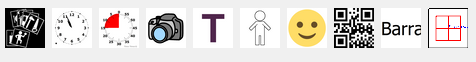
\includegraphics[width=0.7\linewidth]{Imagenes/Bitmap/Ribbon Pictoselector}
	\caption{Barra de inserción de pictogramas.}
	\label{fig:ribbon-pictoselector}
\end{figure}

% TODO: \usepackage{graphicx} required
\begin{figure}[h!]
	\centering
	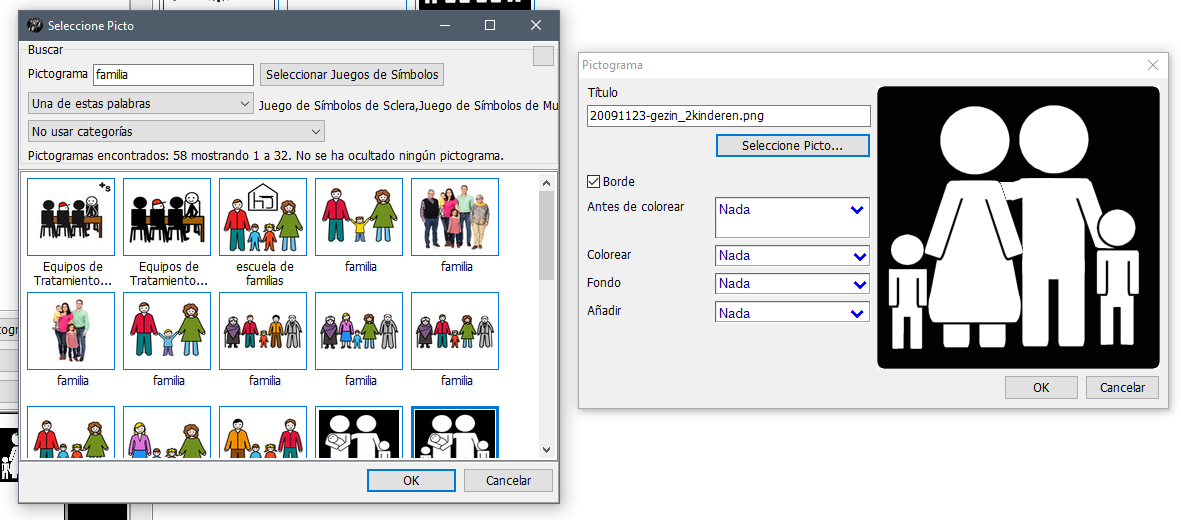
\includegraphics[width=0.7\linewidth]{Imagenes/Bitmap/Editor y buscador de pictoselector}
	\caption{Buscador y editor de Pictogramas.}
	\label{fig:editor-y-buscador-de-pictoselector}
\end{figure}




El mayor inconveniente de la aplicación, pese a ser muy completa respecto a la búsqueda y edición de pictos, es su limitación de colocación a una cuadrícula.

\subsection{Editor ARASAAC}
La página web de ARASAAC cuenta con herramientas online las cuales podemos usar para generar materiales .
\begin{itemize}
\item \textbf{Creador de animaciones}: genera una animación con los pictogramas que queramos en formato GIF o SWF. También permite configurar el intervalo entre los pictogramas y el número de repeticiones que hará.

\item \textbf{Creador de símbolos}: permite la personalización de pictogramas donde podremos cambiar el nombre del pictograma, poner su traducción, modificar la fuente del texto, poner un marco, ampliar la imagen y cambiar el fondo.

\item \textbf{Generador de frases}: consta de un total de tres pasos a seguir, el primero de ellos consiste en seleccionar las palabras que queramos traducir a pictogramas, el segundo paso nos mostrará todos los pictogramas asociados para cada palabra introducida y deberemos seleccionar el que más nos guste y el tercer paso aparecerán todos los pictogramas colocados en una tabla la cual podremos modificar.
\footnote{\url{ http://www.arasaac.org/herramientas.php }}

% TODO: \usepackage{graphicx} required
\begin{figure}[h!]
	\centering
	
\includegraphics[width=0.7\linewidth]{Imagenes/Bitmap/Frase ARASAAC}
	\caption{Ejemplo con generador de frases.}
	\label{fig:frase-arasaac}
\end{figure}


\item \textbf{Generador de horarios}: genera un horario donde previamente tendremos que configurar una plantilla con los días, horas, el formato (horizontal o vertical), idioma, bordes del horario, texto para cada día y hora y la opción de insertar un pictograma en función de su día y hora.

\item \textbf{Generador de calendarios}: genera un calendario donde tendremos que especificar el mes, año e idioma deseado. Al igual que en el generador de horarios permite la opción de modificar el texto, colores, bordes y la posibilidad de poner un pictograma para cada día del mes.

\item \textbf{Generador de tableros}: crea un tablero con el número de filas y columnas deseado donde para cada casilla podremos insertar un pictograma. Al igual que en otras herramientas permite la modificación de colores, bordes y  texto del tablero.

\item \textbf{Creador de juegos}: genera una plantilla en formato .rtf para poder jugar al bingo, oca, dominós y dominós encadenados con los pictogramas que deseemos.
\end{itemize}

% TODO: \usepackage{graphicx} required
\begin{figure}[h!]
	\centering
	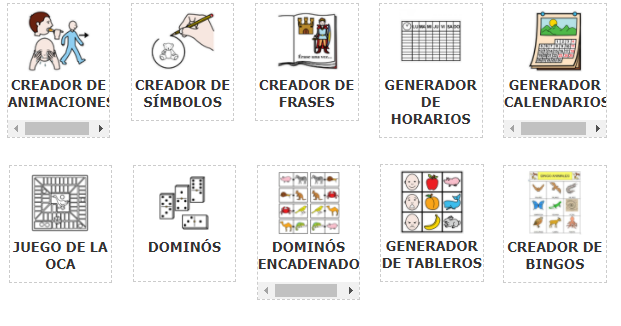
\includegraphics[width=0.7\linewidth]{Imagenes/Bitmap/Tableros ARASAAC}
	\caption[Tableros web ARASAAC]{Herramientas online que ofrece ARASAAC.}
	\label{fig:tableros-arasaac}
\end{figure}

\newpage
\subsection{Piktoplus}
Se trata de una aplicación para dispositivos Android. Su particularidad es que permite la creación de un avatar tridimensional personalizable. Dicho avatar será usado en los tablero pictográficos pues será quien protagonice las acciones. Permite registrar múltiples usuarios, cada uno con su propio avatar. Otra particularidad de Piktoplus son los sub-tableros, por ejemplo, en la Figura \ref{fig:piktoplus1} podemos ver que si se pulsa sobre “Estoy”, se despliega otro tablero con sentimientos, representados con el avatar.

\footnote{\url{http://www.aulautista.com/2013/12/05/piktoplus-un-comunicador-android-muy-especial/ }} \footnote{\url{https://fatimamikel.wordpress.com/2014/04/17/piktoplus-2/ }}
% TODO: \usepackage{graphicx} required
\begin{figure}[h!]
	\centering
	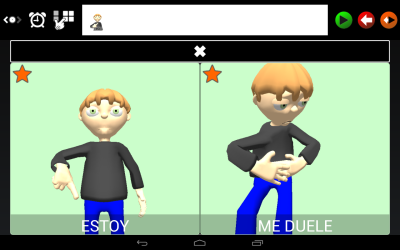
\includegraphics[width=0.7\linewidth]{Imagenes/Bitmap/Piktoplus1}
	\caption[Pictoplus tablero]{Ejemplo de tablero en Piktoplus}
	\label{fig:piktoplus1}
\end{figure}



Respecto a la creación y edición de tableros, se trata de una cuadrícula sobre la cual se colocan los pictos, además permite aumentar el tamaño de los pictos. Por ejemplo “Estoy” ocupa cuatro celdas más que “Contento”.

% TODO: \usepackage{graphicx} required
\begin{figure}[h!]
	\centering
	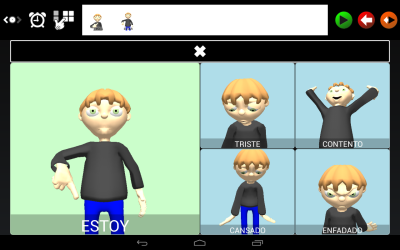
\includegraphics[width=0.7\linewidth]{Imagenes/Bitmap/Piktoplus2}
	\caption[Subtablero Piktoplus]{Subtablero en Piktoplus}
	\label{fig:piktoplus2}
\end{figure}


Actualmente esta aplicación no está disponible para descargar en tiendas de aplicaciones  habituales y su desarrollo ha cesado desde 2018.

\subsection{Pictar}
La aplicación Pictar permite generar una secuencia de pictogramas traduciendo una frase introducida por el usuario. Esa secuencia de pictogramas se podrán colocar automáticamente en el tablero.


El tablero está compuesto por casillas, separadas en filas y columnas permitiendo añadir más elementos.

En el tablero tendremos únicamente la opción de eliminar la casilla o borrar su contenido.En el lateral izquierdo se encuentra un buscador de pictogramas de la base de datos de ARASAAC. Los cuales se pueden colocar en el tablero ya sea sustituyendo pictogramas existentes o rellenando casillas vacías.
\footnote{\url{ http://hypatia.fdi.ucm.es/pictar/ }}

% TODO: \usepackage{graphicx} required
\begin{figure}[h!]
	\centering
	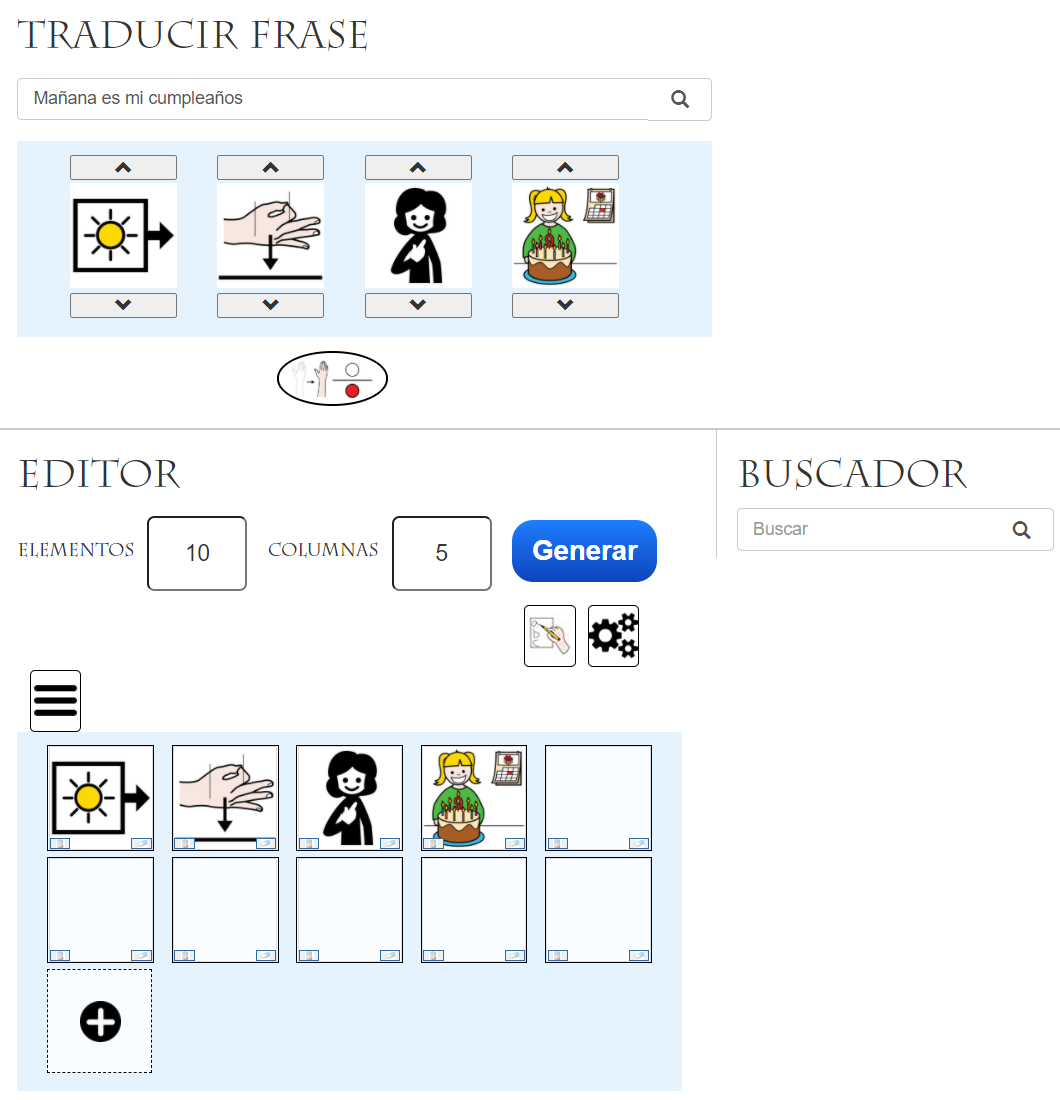
\includegraphics[width=0.7\linewidth]{Imagenes/Bitmap/Pictar}
	\caption{Menú de la aplicación Pictar.}
	\label{fig:pictar}
\end{figure}

\newpage
\subsection{Pictableros}
\footnote{\url{ https://holstein.fdi.ucm.es/picto-tableros/  }}
Pictableros es una aplicación web de edición y creación de tableros y plantillas para pictogramas. Tiene dos partes diferenciadas:

\begin{itemize}
	\item Las plantillas sirven para que otros usuarios que quieran crear un tablero similar puedan sustituir con facilidad los pictogramas. Por ejemplo en la Figura \ref{fig:pictableros1} existe una plantilla de tablero para elegir un deporte, dicha plantilla puede ser modificada para sustituir el pictograma de balonmano por tenis. Estas plantillas pueden ser públicas o privadas.
	
	\item Los tableros públicos no pueden ser modificados, aunque  se puede crear una copia de ellos y modificarse para superponer símbolos (Bien, mal, amarillo, azul)
	

\end{itemize}

	% TODO: \usepackage{graphicx} required
	\begin{figure}[h!]
		\centering
		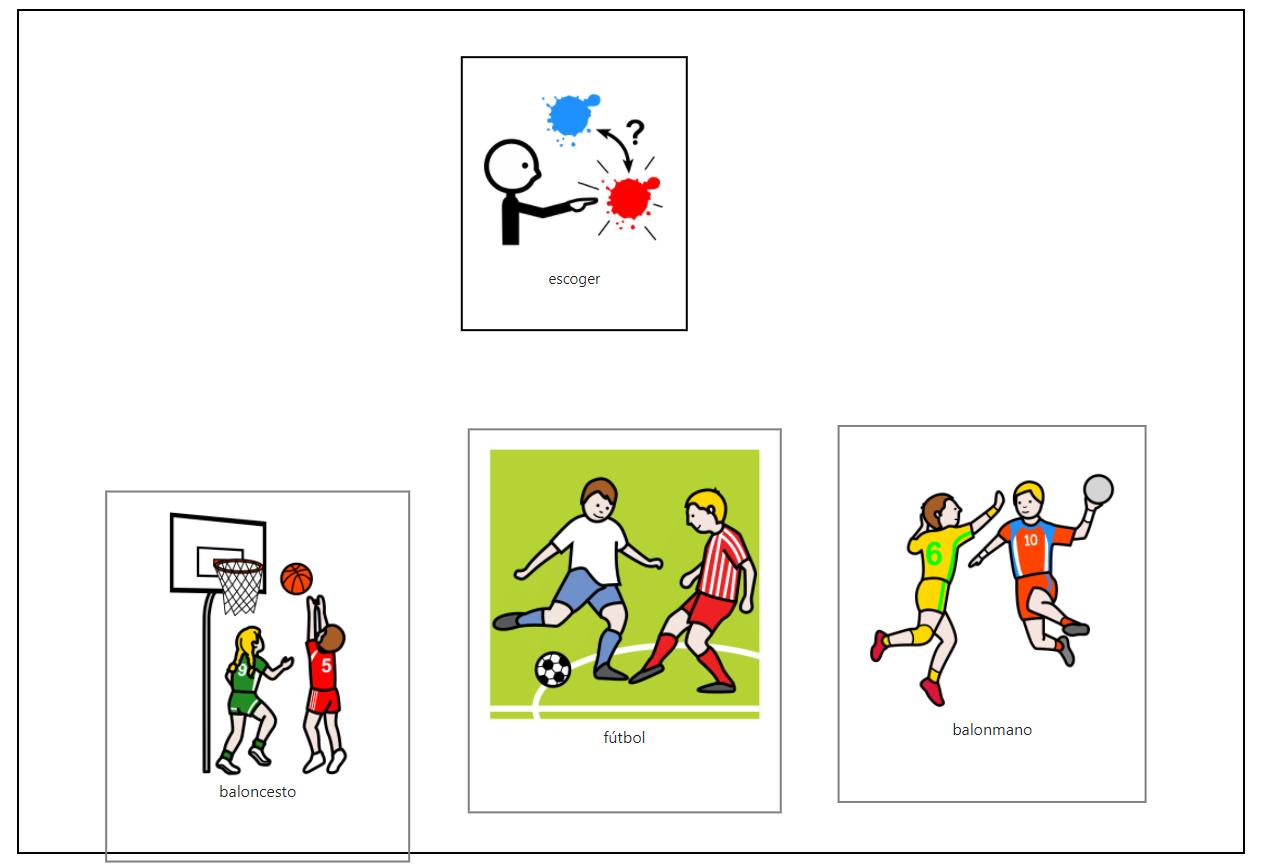
\includegraphics[width=0.7\linewidth]{Imagenes/Bitmap/pictableros1}
		\caption{Plantilla de elección de deporte.}
		\label{fig:pictableros1}
	\end{figure}
	
	
	% TODO: \usepackage{graphicx} required
	\begin{figure}[h!]
		\centering
		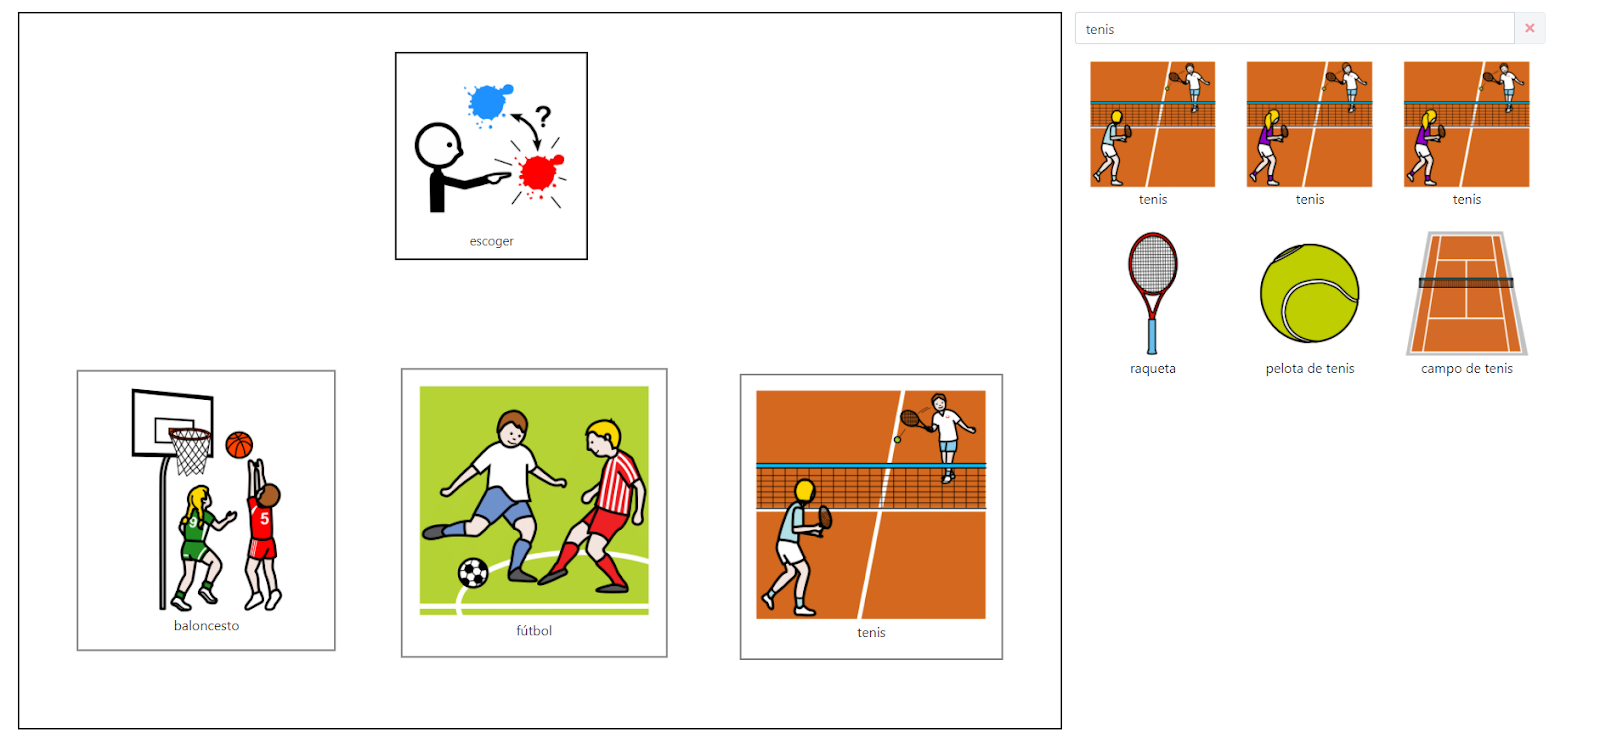
\includegraphics[width=0.7\linewidth]{Imagenes/Bitmap/pictableros2}
		\caption[Edición de plantilla en Pictableros]{Edición de plantilla de selección de deporte, sustituimos balonmano por tenis, haciendo uso del buscador de pictogrmas.}
		\label{fig:pictableros2}
	\end{figure}
	
	% TODO: \usepackage{graphicx} required
	\begin{figure}[h!]
		\centering
		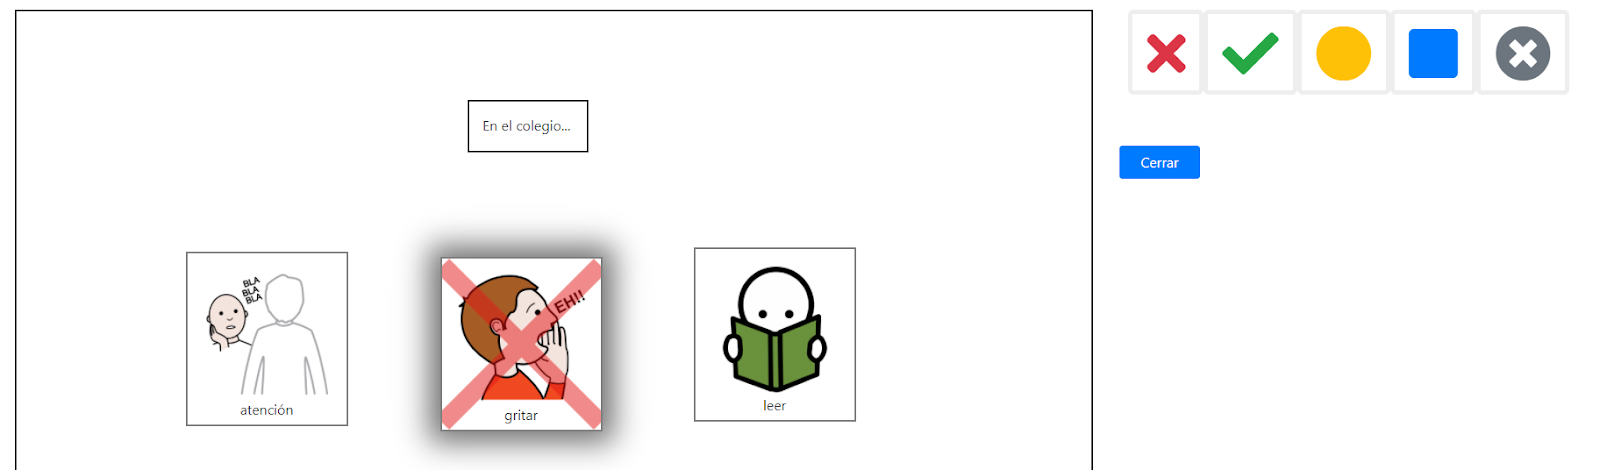
\includegraphics[width=0.7\linewidth]{Imagenes/Bitmap/pictableros3}
		\caption[Edición plantilla en Pictableros]{Edición de tableros, permite superponer un signo al pictograma.}
		\label{fig:pictableros3}
	\end{figure}
	

	


\newpage	
\subsection{Symbo Talk}

SymboTalk permite la creación de tableros de comunicación aumentativa y locución de tableros y pictogramas mediante su aplicación web o dispositivos móviles como Android e iOS.
\footnote{\url{  https://civat.es/app/symbo-talk/ }}
\footnote{\url{   http://aulaabierta.arasaac.org/symbotalk-0-inicio-2  }}
SymboTalk ofrece dos modos de usuario:

\begin{itemize}
	\item \textbf{Modo edición}: permite la creación de pictogramas, construir tableros, buscar pictogramas en un buscador. También ofrece la opción de crear un perfil y poder guardar todos los tableros que hayamos realizado.
	
	\item \textbf{Modo usuario}: pensado para que el usuario pueda comunicarse de una forma más fácil e intuitiva.
	
\end{itemize}

% TODO: \usepackage{graphicx} required
\begin{figure}[h!]
	\centering
	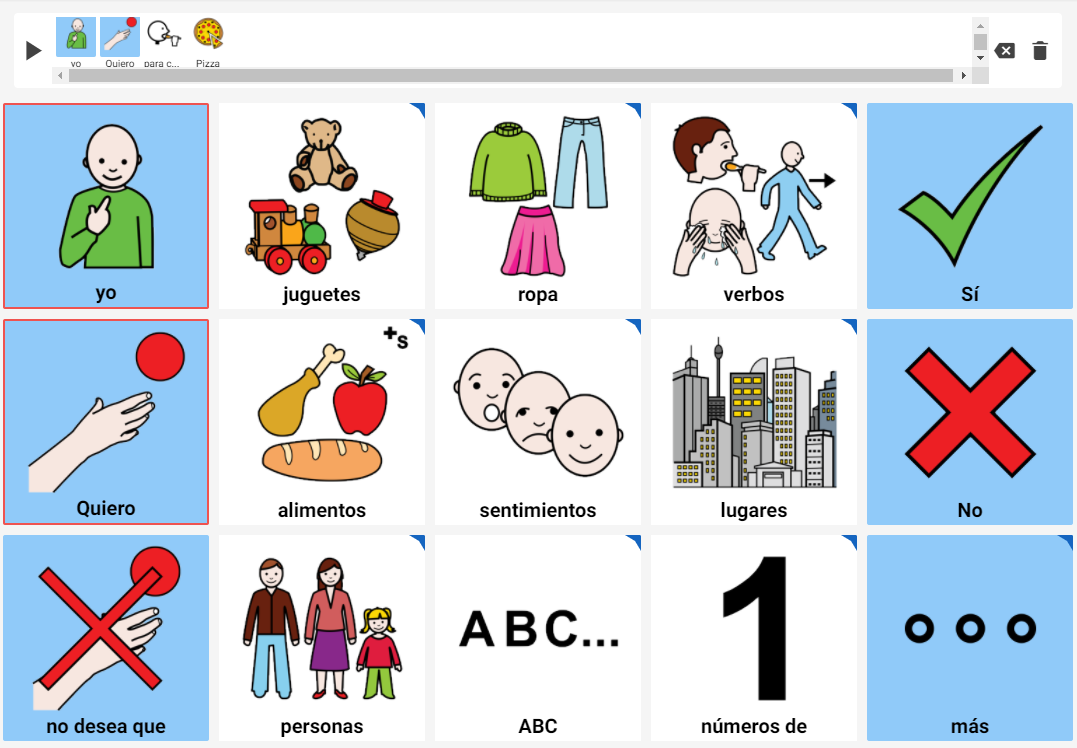
\includegraphics[width=0.7\linewidth]{Imagenes/Bitmap/SymboTalk}
	\caption{Pantalla principal de la aplicación Symbo Talk.}
	\label{fig:symbotalk}
\end{figure}

\newpage
\subsection{LetMe Talk}

LetMe Talk es una aplicación para dispositivos Android e iOS que permite generar frases a partir de pictogramas seleccionados. Tiene un total de 9.000 pictogramas de \textit{ARASAAC} y ofrece la posibilidad de añadir imágenes con un texto descriptivo con la cámara del dispositivo.

\footnote{\url{ https://www.letmetalk.info/es}}
% TODO: \usepackage{graphicx} required
\begin{figure}[h!]
	\centering
	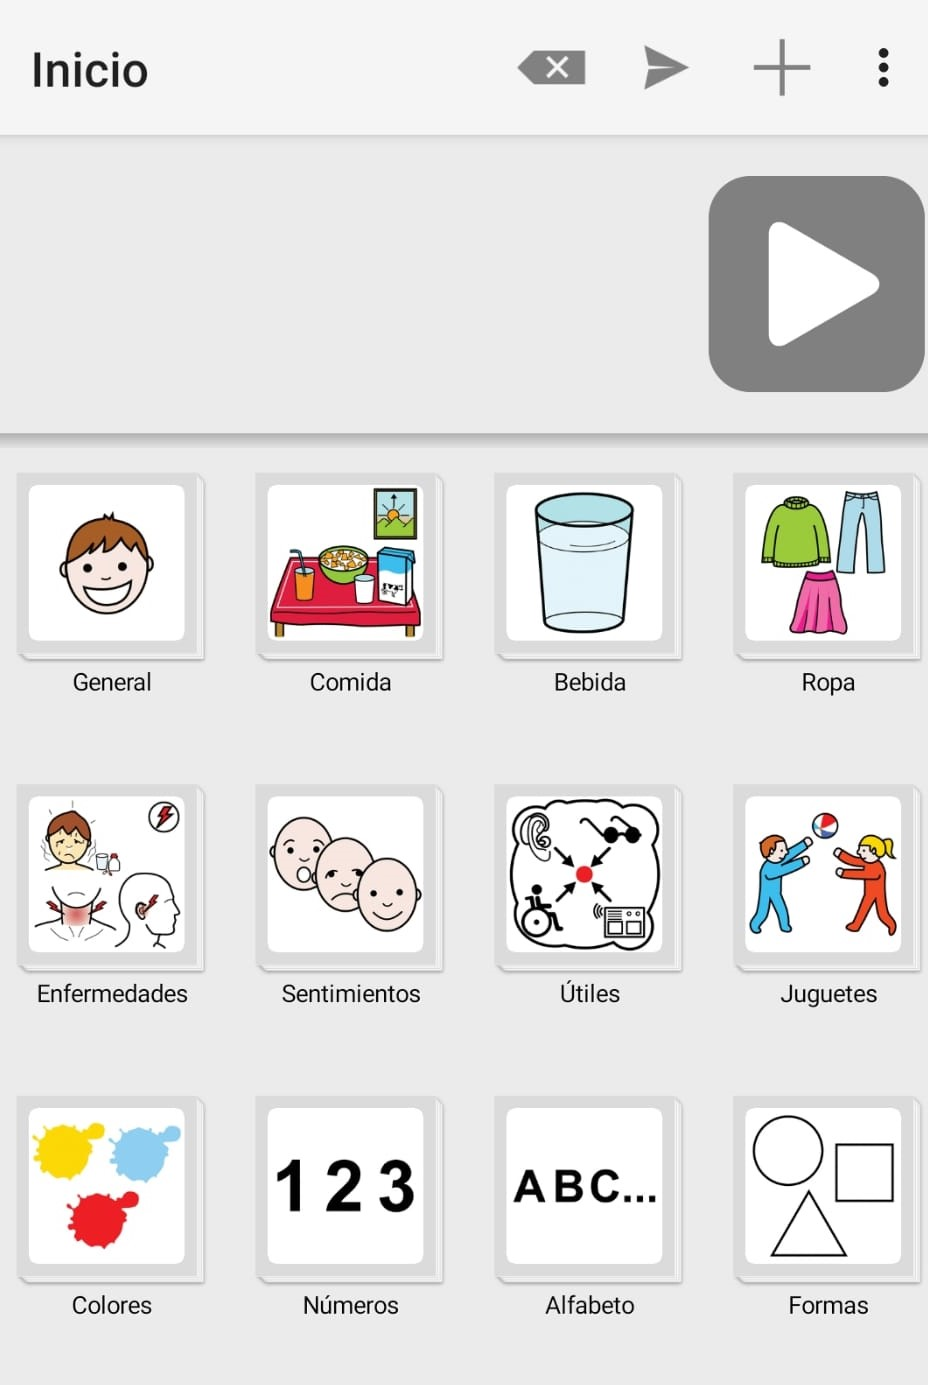
\includegraphics[width=0.7\linewidth]{Imagenes/Bitmap/LetMeTalk}
	\caption{Menú de la aplicación en Android de LetMe Talk.}
	\label{fig:letmetalk}
\end{figure}

\newpage


\begin{table}[]
	\centering
	\resizebox{14cm}{!} {
		\begin{tabular}{|l|l|l|l|l|l|l|}
			\hline
			
			\textbf{Programas} & \textbf{Disponible} & \textbf{Actualizado} & \textbf{Dispositivos} & \textbf{{\begin{tabular}[c]{@{}l@{}}\\ Permite editar \\ pictogramas \\ \\\end{tabular}}}  & \textbf{Precio} & \textbf{Idiomas} \\  \hline
			
			\textbf{Pictoselector} &Si  &Si  &PC y MAC  &Si &Gratuito &{\begin{tabular}[c]{@{}l@{}}\\ES, EN, DU, FR, \\ PT, IT\\ \\\end{tabular}} \\ \hline
			\textbf{Editor ARASAAC} &Si  &Si  &{\begin{tabular}[c]{@{}l@{}}\\PC, MAC, Android, \\ iOS y Web \end{tabular}}  &Si &Gratuito &{\begin{tabular}[c]{@{}l@{}}\\ES, EN, DU, FR, \\ PT, BZ, IT, RO, \\ PL, CN, AR, RU, \\ BG, CRO, NLD\\ \\\end{tabular}} \\ \hline
			\textbf{Piktoplus} &No  &No  &Android  &No &139€ &{\begin{tabular}[c]{@{}l@{}} \\ES \\ \\ \end{tabular}}\\ \hline
			\textbf{BoardMaker} &Si  &Si  &PC y MAC  &No &300€ &{\begin{tabular}[c]{@{}l@{}} \\ES, EN, PT \\ \\\end{tabular}}\\ \hline
			\textbf{Pictar} &Si  &{\begin{tabular}[c]{@{}l@{}}\\La web no, \\los pictogramas si\end{tabular}}  &Web  &No &Gratuito &{\begin{tabular}[c]{@{}l@{}} \\ES \\ \\ \end{tabular}}\\ \hline
			\textbf{Pictableros} &Si  &{\begin{tabular}[c]{@{}l@{}}\\La web no, \\los pictogramas si\end{tabular}}   &Web  &Si &Gratuito &{\begin{tabular}[c]{@{}l@{}} \\ES \\ \\ \end{tabular}}\\ \hline
			\textbf{SymboTalk} &Si  &No  &Web, Android e iOS  &No &Gratuito &{\begin{tabular}[c]{@{}l@{}} \\ES, EN, HEBR \\ \\ \end{tabular}}\\ \hline
			\textbf{LetMeTalk} &Si  &No  &Android e iOS  &No &Gratuito &{\begin{tabular}[c]{@{}l@{}} \\ES, AR, DE, EN, \\ IT, FR, PL, PT, \\ RU, RO, SW, CN \\ \\\end{tabular}} \\ \hline
			
		\end{tabular}
	}
\caption{\label{tab:table-name}Tabla comparativa entre los distintos editores de tableros basados en pictogramas}
\end{table}